\documentclass[12pt,oneside]{book}
\usepackage{times,mathptmx}
\usepackage[pdftex]{graphicx}
\usepackage{calc}
\usepackage{tabularx,ragged2e,booktabs,caption,subcaption}
\usepackage{array}
\newcolumntype{L}[1]{>{\raggedright\let\newline\\\arraybackslash\hspace{0pt}}m{#1}}
\newcolumntype{C}[1]{>{\centering\let\newline\\\arraybackslash\hspace{0pt}}m{#1}}
\newcolumntype{R}[1]{>{\raggedleft\let\newline\\\arraybackslash\hspace{0pt}}m{#1}}
\usepackage{multirow}
\usepackage{multicol}
\usepackage{tocloft}
\usepackage{xcolor}
\usepackage{color,soul}
\usepackage{amsmath}
\definecolor{linknavy}{rgb}{0,0,0.50196}
\definecolor{linkred}{rgb}{1,0,0}
\definecolor{linkblue}{rgb}{0,0,1}
\definecolor{darkorange}{rgb}{0.81,0.52,0}
\definecolor{fc_orange}{rgb}{0.94,0.59,0.14}
\definecolor{brown}{rgb}{0.56,0.36,0}
\definecolor{fc_blue}{rgb}{0.27,.36,0.48}
\usepackage{float}
\usepackage{graphpap}
\usepackage{rotating}
\usepackage{graphicx}
\usepackage{geometry}
\usepackage{relsize}
\usepackage{ltablex}
\usepackage{longtable}
\usepackage{lscape}
\usepackage{amssymb}
\usepackage{makeidx} % Create index at end of document
\usepackage[nottoc,notlof,notlot]{tocbibind} % Put the bibliography and index in the ToC
\usepackage{lastpage} % Automatic last page number reference.
\usepackage[T1]{fontenc}
\usepackage{enumerate}
\usepackage{upquote}
\usepackage{moreverb}
\usepackage{xfrac}
\usepackage{cite}
\usepackage{tikz}
% \usepackage{subfig}
% \usepackage{caption}
\usepackage[toc,page]{appendix}
\usepackage{notoccite}
\usepackage{placeins}

\usepackage{titlesec}
\titleformat{\chapter}[hang] 
{\color{fc_blue}\normalfont\huge\bfseries}{\chaptertitlename\ \thechapter}{1em}{}[\titlerule]
\titlespacing*{\chapter}{0pt}{-30pt}{20pt}

\titleformat*{\section}{\normalfont\Large\bfseries\color{fc_blue}}
\titleformat*{\subsection}{\normalfont\large\bfseries\color{fc_blue}}

\newcommand{\nopart}{\expandafter\def\csname Parent-1\endcsname{}} % To fix table of contents in pdf.

\usepackage{siunitx}
\sisetup{
    detect-all = true,
    input-decimal-markers = {.},
    input-ignore = {,},
    inter-unit-product = \ensuremath{{}\cdot{}},
    multi-part-units = repeat,
    number-unit-product = \text{~},
    per-mode = fraction,
    separate-uncertainty = true,
}

\usepackage{listings}
\usepackage{textcomp}
\definecolor{lbcolor}{rgb}{0.96,0.96,0.96}

\usepackage[pdftex,
        colorlinks=true,
        urlcolor=fc_orange,     % \href{...}{...} external (URL)
        citecolor=fc_orange,     % citation number colors
        linkcolor=fc_orange,    % \ref{...} and \pageref{...}
        pdfproducer={pdflatex},
        pdfpagemode=UseNone,
        bookmarksopen=true,
        plainpages=false,
        verbose]{hyperref}

\renewcommand{\cftchapfont}{\hypersetup{linkcolor=fc_blue}}
\renewcommand{\cftsecfont}{\hypersetup{linkcolor=black}}
\renewcommand{\cftsubsecfont}{\hypersetup{linkcolor=black}}
\renewcommand{\cftsubsubsecfont}{\hypersetup{linkcolor=black}}


\setlength{\textwidth}{6.5in}
\setlength{\textheight}{9.0in}
\setlength{\topmargin}{0.in}
\setlength{\headheight}{0.pt}
\setlength{\headsep}{0.in}
\setlength{\parindent}{0.0in}
\setlength{\itemindent}{0.25in}
\setlength{\oddsidemargin}{0.0in}
\setlength{\evensidemargin}{0.0in}
% \setlength{\leftmargini}{\parindent} % Controls the indenting of the "bullets" in a list
\setlength{\cftsecnumwidth}{0.45in}
\setlength{\cftsubsecnumwidth}{0.5in}
\setlength{\cftfignumwidth}{0.45in}
\setlength{\cfttabnumwidth}{0.45in}
\setlength{\parskip}{1em}

% \newcolumntype{L}{>{\centering\arraybackslash}m{4cm}}

\floatstyle{boxed}
\newfloat{notebox}{H}{lon}
\newfloat{warning}{H}{low}

\newenvironment{conditions}
  {\par\vspace{\abovedisplayskip}\noindent\begin{tabular}{>{$}l<{$} @{${}={}$} l}}
  {\end{tabular}\par\vspace{\belowdisplayskip}}


% Rename chapter headings
\renewcommand{\chaptername}{}
\renewcommand{\bibname}{References}

\usepackage{tikz}
\usetikzlibrary{calc}

\usepackage{fancyhdr}
\pagestyle{fancy}
\lhead{}
\rhead{}
\chead{}
\renewcommand{\headrulewidth}{0pt}


% \usepackage{draftwatermark}
% \SetWatermarkText{DRAFT}
% \SetWatermarkScale{1}

\begin{document}
\pagenumbering{gobble}

\bibliographystyle{unsrt}
%\pagestyle{empty}

\frontmatter

\begin{minipage}{1.0\textwidth}
\pagecolor{fc_blue}
\pagenumbering{gobble}

\vspace{1cm}
\centering

\includegraphics[width=2.5in]{Figures/firecares-header-logo_2}
\noindent\makebox[\linewidth]{\color{white}\rule{.5\paperwidth}{0.6pt}}

\Huge \color{fc_orange} Technical Reference Guide \\

\vspace{0.5cm}

\large{\color{white} Version: 1.5  \hspace{1cm} Compilation Date: \today \\}

\vspace{4cm}

{\Large \em \color{fc_orange}Analyze how fire department resources \\
are deployed to match a community's risks. \\
}
\end{minipage}


\frontmatter
\pagecolor{white}

\newpage
\hspace{5in}
\newpage

\pagestyle{fancy}{
\fancyhf{}
\fancyhead[]{%
   \begin{tikzpicture}[overlay, remember picture]%
   \fill[fc_blue] (current page.north west) rectangle ($(current page.north east)+(0,-.5in)$);
   \node[anchor=north west, text=white, font=\Large\scshape, minimum size=1in, inner xsep=5mm] at (current page.north west) {};
   \end{tikzpicture}
}
\fancyfoot[C]{
   \begin{tikzpicture}[overlay, remember picture]%
   \fill[fc_orange] (current page.south west) rectangle ($(current page.south east)+(0,.5in)$);
   \node[anchor=south west, text=black, minimum size=.5in] at (current page.south west) {\thepage};
   \end{tikzpicture}
}}


\fancypagestyle{plain}{
\fancyhf{}%
% \fancyfoot[C]{\thepage\ of \pageref{LastPage}}%
\fancyhead[]{
   \begin{tikzpicture}[overlay, remember picture]% 
   \fill[fc_blue] (current page.north west) rectangle ($(current page.north east)+(0,-.5in)$);
   \node[anchor=north west, text=white, font=\Large\scshape, minimum size=1in, inner xsep=5mm] at (current page.north west) {};
   \end{tikzpicture}
}
\fancyfoot[C]{
   \begin{tikzpicture}[overlay, remember picture]%
   \fill[fc_orange] (current page.south west) rectangle ($(current page.south east)+(0,.5in)$);
   \node[anchor=south west, text=black, minimum size=.5in] at (current page.south west) {\thepage};
   \end{tikzpicture}
}}


\pagenumbering{roman}

\newpage

\cleardoublepage


% \phantomsection

\renewcommand*\contentsname{\color{fc_blue}Contents}
\tableofcontents

\hypersetup{ 
    linkcolor=fc_orange,         % moved after \tableofcontents
    filecolor=fc_orange,      % 
    urlcolor=fc_orange,           %
}    

\newpage
\mainmatter

\chapter{Community Risk}


\chapter{Fire Department Performance Score}
\section{Meaning of Fire Department Performance}
Before describing in detail the current performance score framework, it is worth discussing the meaning fire department performance. Given the purpose of a fire department, it is reasonable to define performance as the degree to which a department adopts practices that minizmize the likelihood of negative consequences from a fire, specifially deaths, injuries, and property damage. As a thought experiment, one could imagine a world with perfect information an no scarity of data. If this were the case, the performance score could be determined by evaluating every action taken by a fire department and the resulting prevention of loss of life and property damage. In this scenario, the number of prevented casualites and the total amount of prevented damage would serve as meaninful performance metrics. However, in reality, there are several major obscales to this assesment. Firstly, not all actions taken by a fire department for a given fire scenario are reported. Secondly, it is very difficult to quantify the effects of of all actions taken by a fire department, and when negative outcomes occur due to a fire, it is difficult to assess the degree to which these outcomes were the result of fire department performance deficiencies or the result of factors completely outside the control the fire department. For example, let's say two departments, Department A and Department B respond to a fire events respectively. Department A responds to a small trash can fire that does not spread beyond its item of origin, but the department shows up to the scene very late, and the firefighters cannot connect the hose quickly due to lack of training. On the other hand, Department B promptly shows up to an upholstered furniture fire that quickly flashes over the room and causes significant property damage despite the fact that the firefighters arrived quickly and estinguished the fire with efficacy. If one were to compare the performance of the two departments based purely on the outcomes, then Department A would be evaluated more favorably, despite the fact that the difference in damage between the two scenarios is entirely due to factors that are outside the fire departments' control. 

In spite of the dearth of perfect information and reporting, many simple metrics exist that can be used to gauge the relative performance of fire departments. For example, the percentage of emergency incidents whose response time falls below a certain value, the number of unintentional fire deaths occurring in structures, or the percent of structure fires confined to room of origin are all used as metrics to judge a fire department's performance. Aside from arrival time metrics, such metrics do not necessarily inform a fire department as to the effectiveness of their training and/or tactics because they do not supply a standard of comparison. For example, if 40\% of the structure fires a fire department responds to spread beyond the room of origin, it is unclear whether this is due to the fire department, or due to the types of fuel loads present in its community. There is a clear metric, time to arrival, that informs a fire department as to how it needs to train for response time, and what is missing regarding the speed at which they respond to an incident. Metrics as clear as time to arrival do not presently exist for determining quality of training and tactics regarding fire suppression. FireCARES employs a new metric, dubbed the tactical correction time (TCT), to aid in quantifying fire department tactical effectiveness. The concept is that there exists some TCT for all fire department structure fire responses that, in lieu of national standards governing response times and routed through a simple fire damage model, ``corrects'' the fire damage outcomes expected from national standards to the particular outcomes observed by a given fire department.  Here, ``fire damage outcomes'' refers to the structure fire spread category from the National Incident Reporting System (NFIRS), which rates the fire spread in a structure from ``confined to object of origin'' through ``spread beyond structure of origin.'' The ``departure'' of a fire department's fire damage outcomes from those outcomes expected using national standards and a simple flame damage model provides an assessment metric that can identify where a given fire department's training might be lacking, or where suppression tactics might be improved. Finally, this metric is further processed under assumptions that supply a single-number metric, a ``fire department performance score.''

\section{Motivation}
The goal of this model is to develop and estimate a new performance metric for fire departments, in time response form, that will aid them in disambiguating their suppression training from their response time training. Presently, various standards exist for fire department response times, courtesy of the NFPA among other organizations. These standards, developed by committees of fire protection professionals, are assumed to encode the societal expectations placed on fire departments with respect to various aspects of their operations, and provide a useful bar against which fire departments can examine the efficacy of their training regimes. For example, the NFPA 1710 standard dictates a distribution of acceptable timings for dispatches, turnout time, and arrival time to incidents. If a fire department finds they fail to meet the standard with regards to, say, turnout time, they can choose to conduct training with their personnel to ensure that this ideal target is obtained.

Unfortunately, an analogue to such useful metrics does not appear to exist for supplying fire departments feedback on their suppression tactics during operations. The model to be presented attempts to rectify this situation by relating the expectations of fire department constituencies, codified in the form of ``national standards,'' observational output regarding a fire department's actual ``performance'' in suppressing fires, and the characteristics of the community that a given fire department serves that may affect this performance using a simple relational model.

The end result of such modeling is to obtain a ``Tactical Correction Time,'' which is interpreted as the departure, measured in seconds, of a given fire department from the expectations placed upon it by national standards when ``suppressing'' a fire representative of a given occupancy type. This metric is thus intended to aid fire departments in identifying whether their fire suppression operations are performing according to the expectations placed upon them, or whether there is an apparent departure from expectation that could indicate improvements could be made through training or other adjustments.

\section{TCT model}
Figure~\ref{fig:TCTforward} outlines the conditional model in a forward sense, where tactical correction time is assumed known and . As can be seen, the relational model is a simple exponential area damage model the form of which is consistent with fire statistics literature. For this model, the value of $A(0)$ was fixed at 1 sq. ft., assumed as an ``established burning'' fire, and $\theta$ was selected to constrain the total area damaged by the fire to exceed the area of the estimated average size of compartments in U.S. residential homes within 10 minutes.

\begin{figure}[htb]
  \centering
  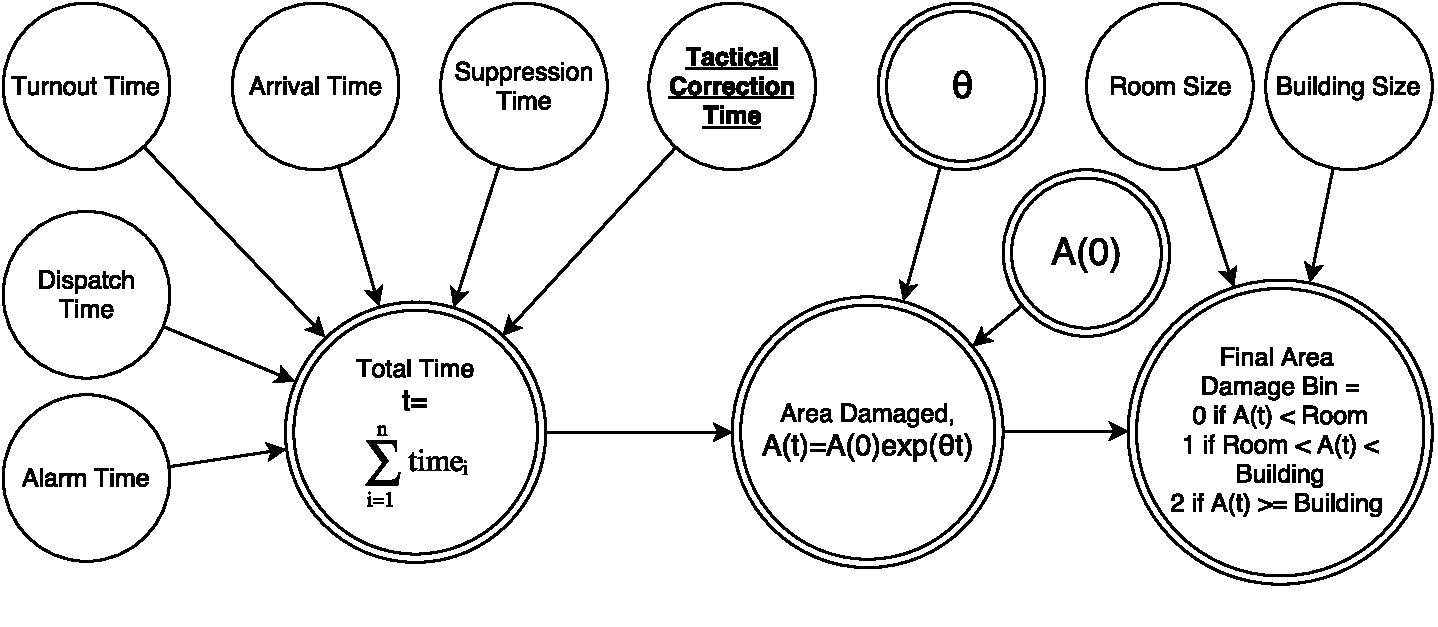
\includegraphics[width=0.95\textwidth]{./Figures/TCTforward}
  \caption{TCT forward model conditional relations. Items within circles denote uncertain quantities, Items within double-circles denote deterministic quantities or transformations.}
  \label{fig:TCTforward}
\end{figure}

For building structure fire responses, NFIRS records an ``extent of fire spread'' field, indicating whether a fire was confined to its ``room of origin,'' its ``building of origin,'' or whether it ``spread beyond the building of origin.'' Let A(t) denote the area damaged by a fire, as given by Fire size in figure~\ref{fig:TCTforward}. In that case, Final Area Damage Bin is defined as follows:
 \begin{displaymath}
   Bin = \left\{
     \begin{array}{lr}
       \text{Contained to Room} &  A(0) <= A(t) <= \text{Room size}\\
       \text{Contained to Bldg} &  \text{Room size} < A(t) < \text{Bldg size}\\
       \text{Spread Beyond Bldg} & A(t) = \text{Bldg size}\\
     \end{array}
   \right.
\end{displaymath} 

The assertion regarding Spread beyond building may seem peculiar. The assumption here is that the total damaged area of a fire that is classified as ``spread beyond the building of origin'' is constrained to simply be the area of the building. This assumption is necessary to provide a reasonable upper bound to the tactical correction time for fires that are spread beyond the room of origin. 

Figure~\ref{fig:TCTinverse} displays the conditional relations of the model if it is inverted such that the value being derived is tactical correction time. In order to derive this quantity, the following assumptions are made:
\begin{itemize}
  \item The distributions related to Alarm, Arrival, Suppression, Dispatch, and Turnout time, as well as room and building size, are all mutually independent and known.
  \item A(0) and $\theta$, as described above, are fixed.
  \item In the inversion case, the inversion of the binning function using drawn room and building sizes coupled with observed bins implies a range of possible values for area damaged. Because no other information is used in determining the size of the fire in the inverse sense, the distribution of ``Area damaged''  is assumed to be uniformly distributed between the constraints imposed by the observed damage bin and the room and building sizes. 
    Formally:
    \[f_A(a|Bin,A_{room},A_{bldg}) \sim 
      \begin{cases}
  Unif(A(0),A_{room}) \quad Bin = 0 \\
  Unif(A_{room},A_{bldg}) \quad Bin = 1 \\
  A_{bldg} \quad Bin = 2 
      \end{cases}
    \]
\end{itemize}

\begin{figure}[htb]
  \centering
  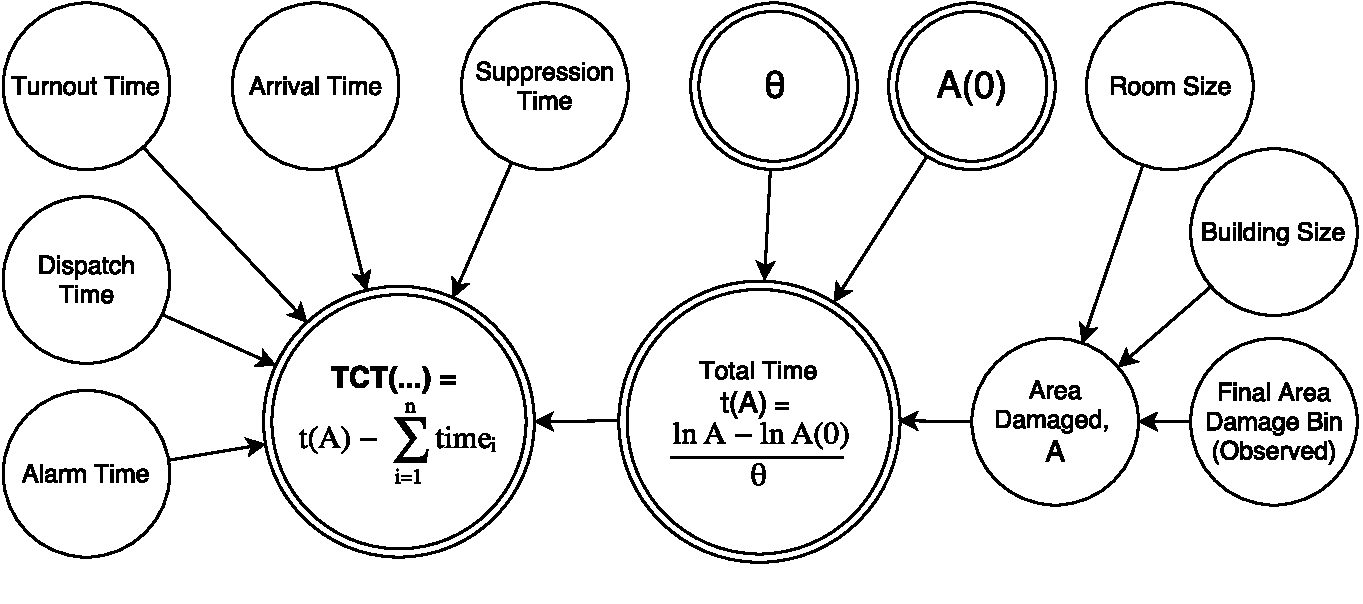
\includegraphics[width=0.95\textwidth]{./Figures/TCTinverse}
  \caption{Inversion model taking final area damage bins from real fire data and inverting for TCT.}
  \label{fig:TCTinverse}
\end{figure}

Using these assumptions, it is possible to derive a gibbs sampler that can perform posterior draws on TCT given actual fire spread outcome data. For this derivation, Table~\ref{tab:terminology} supplies the glossary of variables. A gibbs sampler is a subset of the metropolis hastings algorithm, which attempts to perform monte carlo draws from the joint distribution of all stochastic variables in a model. These draws can then be used to derive estimates of parameters of interest and their uncertainty from a model.

\begin{table}[htb]
  \centering
  \caption{Glossary of terms used in inverse TCT model}
  \begin{tabular}{lp{4cm}}
    $t_{al}$ & alarm time \\
    $t_{di}$ & dispatch time \\
    $t_{to}$ & turnout time \\
    $t_{ar}$ & arrival time \\
    $t_{su}$ & suppression time \\
    $t_{tct}$ & tactical correction time (TCT)\\
    $t_{tot}$ & total fire growth time\\
    $A_{room}$ & Floor area of room \\
    $A_{bldg}$ & Floor area of building \\
    $A$ & Area damaged by fire \\
    $A(0)$ & Area damaged by fire at ``established burning'' \\
    $\theta$ & Area damage propagation rate \\
    $Bin$ & Observed fire spread category of individual fire \\
  \end{tabular}
  \label{tab:terminology}
\end{table}

From the assumptions stated above, the distributions of the fire department timing variables are assumed to be independently distributed, with their distributions according to either expert judgment, national standard, or historical timing data where available. Likewise, the distributions of the room and building sizes are estimated from the American Housing Survey's national survey of residential homes. Where available, it is possible to use the AHS metropolitan statistical areas to refine room and building distributions for larger metropolitan areas. For purposes of showing the derivation, these timing and building distributions are assumed to be uniformly distributed according to parameters $a_i$ and $b_i$ where $i$ is the particular variable name. Thus:
\begin{alignat*}{3}
  t_{al}|\dots &\sim t_{al} &\sim& Unif(a_{al},b_{al}) \\
  t_{di}|\dots &\sim t_{di} &\sim& Unif(a_{di},b_{di}) \\
  t_{to}|\dots &\sim t_{to} &\sim& Unif(a_{to},b_{to}) \\
  t_{ar}|\dots &\sim t_{ar} &\sim& Unif(a_{ar},b_{ar}) \\
  t_{su}|\dots &\sim t_{su} &\sim& Unif(a_{su},b_{su}) \\
  A_{room}|\dots &\sim A_{room} &\sim& Unif(a_{room},b_{room}) \\
  A_{bldg}|\dots &\sim A_{bldg} &\sim& Unif(a_{bldg},b_{bldg}) 
\end{alignat*}
where $\dots$ indicates conditionality on all other variables within the model. The full conditional distributions of the above variables are equivalent to their marginal distributions due to the assumption of mutual independence. Next, the full conditional distribution of Area damaged by fire is outlined in the assumptions above. It consists of three possible uniform distributions based on partitions dictated by the observed fire spread category and a given room and building size. From these distributions, obtaining a value of TCT is a strict transformation based on given values, whose derivation is outlined in Figure~\ref{fig:TCTinverse}, but also supplied below using the variables in Table~\ref{tab:terminology}:
\begin{equation}
  \label{eqn:tctinverse}
  t_{tct} = \left(\frac{\ln A - \ln A(0)}{\theta}\right)-\left(t_{al}+t_{di}+t_{to}+t_{ar}+t_{su}\right)
\end{equation}

Thus, the form of the gibbs sampler is as follows:
\begin{enumerate}
  \item Draw values for fire department timing and room and building size variables.
  \item Draw value for area damaged given observed fire spread category bin and room and building size variables
  \item Compute value of TCT given above variables using Equation~\ref{eqn:tctinverse}.
\end{enumerate}

Note that the model outlined above would require a number of chains equal to the number of fire incidents whose fire spread category is known in order to run. However, observing how area damaged by a fire is drawn based on fire spread category, it is possible to simplify the model computationally with a few observations.

\begin{figure}[htb]
  \centering
  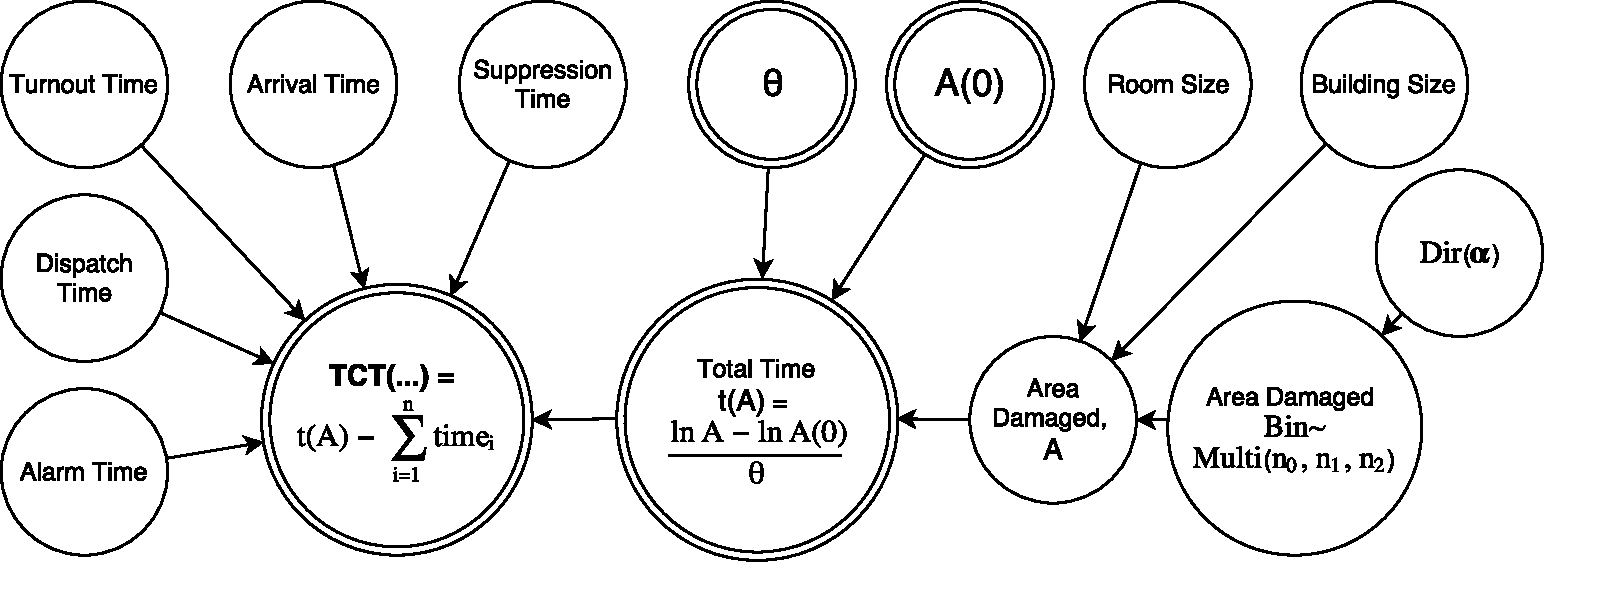
\includegraphics[width=0.95\textwidth]{./Figures/TCTinversemulti}
  \caption{Inversion model with multinomial distribution assumption placed upon final area damage bins, along with non-informative Dirichlet prior.}
  \label{fig:TCTinversemulti}
\end{figure}

First, due to the assumptions surrounding the distribution of $A$, it is apparent that the posterior distribution of TCT from the inverse model is actually just a mixture of 3 different distributions, each associated with a fire spread category. In other words, for a given fire, the observed data only affects the partition on area damaged by fire. Thus, it is possible to reduce the number of necessary running chains to 1 from $N$, where $N$ is the total number of observed fires, by assuming that the fire spread categories are multinomially distributed, a reasonable assumption given that the data is categorical in nature. This change affects the inversion model according to figure~\ref{fig:TCTinversemulti}. Namely, the assumption that the bin observations are distributed multinomially, coupled with a non-informative dirichlet prior, implies a Dirichlet posterior distribution can be drawn from for the binning. The derivation is a conjugate derivation and so can be found in most bayesian analysis textbooks, for example \cite{Gelman2013}, but is included here to provide some exposure to the procedure:

Because the goal of this analysis is to derive a posterior distribution from a conjugate prior, the focus is on the \emph{kernel} of the distributions involved, and thus only proportionality with regards to the underlying parameter of interest, here the vector of probabilities for the underlying multinomial distribution of the observations, is necessary. For this analysis, this parameter is $\mathbf{\theta}=(\theta_1,\theta_2,\theta_3)$.

First, we assert that the fire spread data is multinomial as follows:
\[
  p(y|\theta) \propto \prod^k_{j=1} \gamma_j^{y_j}
\]
Where $y_j$ is the count of fires observed in bin $j$ (here an observed final damage bin/fire spread category) and $\theta$ is as described above, subject to the following constraints:
\[
  \sum_{j=1}^k\theta_j = 1
  \sum_{j=1}^k y_j = n
\]
where $n$ is in this model the total number of residential building fires with recorded fire spread categories. The conjugate prior distribution to the multinomial is the Dirichlet distribution,
\[
  p(\theta|\alpha) \propto \prod_{j=1}^k \theta_j^{\alpha_j-1}
\]

Since this distribution is a prior, it represents our prior belief about the underlying distribution of the probability of a given fire belonging to a given fire spread category. An example of a ``non-informative prior'' in this situation would be $\mathbf{\alpha}=(\alpha_1,\alpha_2,\alpha_3)=(1,1,1)$ such a prior adds the equivalent of one observation to each category uniformly.

Now consider Bayes' rule:
\[
  p(\theta|y,\alpha) = \frac{p(y|\theta,\alpha)p(\theta|\alpha)}{p(y,\alpha)}
\]

The parameters in the denominator are known, (either assumed or observed), and thus it is known that $p(y,\alpha)$ is a constant used to ``renormalize'' the distribution to integrate to 1, but actual evaluation of that constant is non-trivial. Thus, we proceed as stated above using proportionality in the hope of ``discovering'' the kernel of a distribution that is known:
\begin{align*}
  p(\theta|y,\alpha) &\propto p(y|\theta)p(\theta|\alpha)
  &\propto \prod^k_{j=1} \gamma_j^{y_j}\prod_{j=1}^k \theta_j^{\alpha_j-1} 
  &\propto \prod_{j=1}^k \theta_j^{(\alpha_j+y_j)-1}
\end{align*}

From the final expression, note that it would be possible to redefine $\alpha_j+y_j$ as $\alpha'$, and the expression would be the kernel of a $Dirichlet(\mathbf{\alpha}')$ distribution. Thus, the posterior distribution is Dirichlet with parameters $\alpha_j+y_j$.

With this derivation in hand, the modification to the gibbs sampler now appears as follows:
\begin{enumerate}
  \item Draw values for fire department timing and room and building size variables.
  \item Draw values for $\theta$ from the posterior distribution above
  \item Draw a bin value from the multinomial($\mathbf{\theta}$) with n=1. Note that this distribution is the posterior predictive distribution of the observations, $p(\tilde{y}|y)$.
  \item Draw value for area damaged given observed fire spread category bin and room and building size variables
  \item Compute value of TCT given above variables using Equation~\ref{eqn:tctinverse}.
\end{enumerate}

\section{Condensing the TCT distribution into a fire department performance metric}
While a distribution on performance is valuable, philosophically it is not fully clear whether a fire department should be recompensed in the same manner for arriving well ahead of schedule versus arriving very late to a fire.

The decision was made to develop a metric that focused solely on the positive side of the TCT distribution. Thus, one additional modification was made to the gibbs sampler as a post-processing step: All negative TCT values were truncated to zero. Note that such a change does not neglect or remove these distribution draws, but simply alters the overall distribution to include an additional point-mass at zero representing the total probability of the fire department responding in a manner commensurate with national standards or an ``ideal'' version of itself, should the fire department's own timing distributions be used. Mathematically, this is one more transformation that augments TCT to be strictly positive, thus emphasizing the aspect of improvement potential. 

Figure~\ref{fig:normtruncexample} shows an example of this procedure applied to the standard normal distribution. There is a 0.5 probability that a draw from the distribution will be negative. Thus, when all negative values are truncated to zero, this puts a 0.5 probability mass upon zero, with the positive portion of the distribution remaining intact.

\begin{figure}[htbp]
  \centering
  \begin{subfigure}[t]{0.45\textwidth}
      \centering
      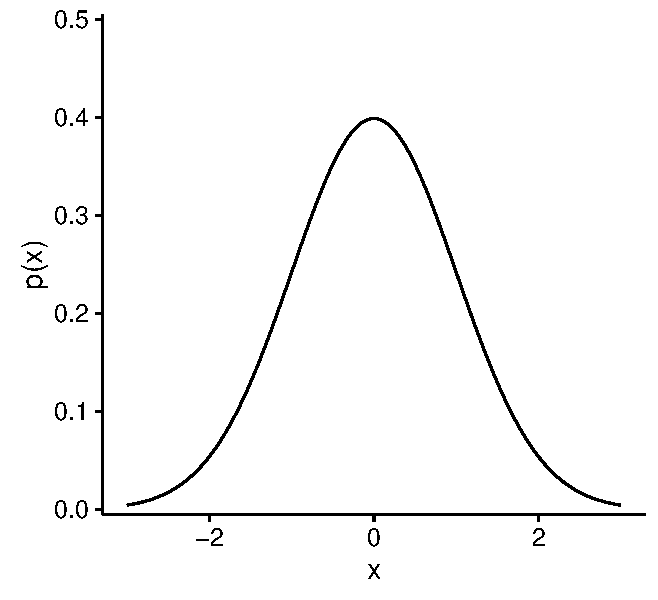
\includegraphics[width=\textwidth]{./Figures/normgraph}
      \caption{Standard normal distribution}
  \end{subfigure}
  \begin{subfigure}[t]{0.45\textwidth}
      \centering
      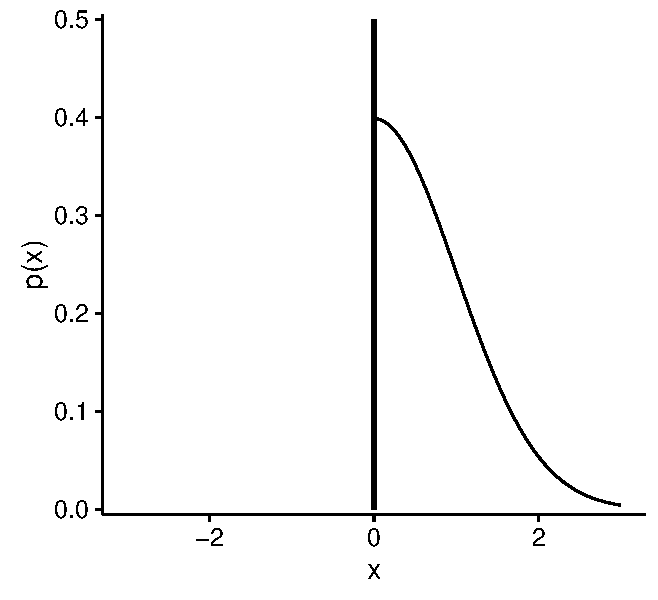
\includegraphics[width=\textwidth]{./Figures/truncgraph}
      \caption{Standard normal distribution truncated at zero}
  \end{subfigure}
  \caption{Application of truncation procedure to standard normal distribution. Note that the bar in (b) indicates a probability mass located at zero.}
  \label{fig:normtruncexample}
\end{figure}

Finally, a simple performance metric is defined from the the truncated TCT distribution as the average of the distribution. This metric is deemed the ``Fire department performance score.''

\section{Drawn parameters}
\subsection{Room areas}
\subsection{Building areas}
The defaults for floor area and building area are also modified in the medium and high hazard DIST models. In this write-up and within the model, floor area refers to the square footage of an individual unit or apartment.  Building area refers to the total plan area of all units on a floor of a building. This convention was chosen to best describe the NFIRS designation of fire spread beyond building for medium and high hazard structures.  For these types of structures, we believe that a fire affecting multiple units would most likely be described as having spread beyond the floor, and one that affects all units on the story would be designated as having spread beyond the building.  The default floor area draw is now a custom draw based on the reported unit square footages of respondents who live in buildings with 3-7 stories for the medium hazard model and 8 or more stories for the high hazard model. As previously noted, the building area corresponds to the area of a story of a medium or high hazard building. Because this figure is not reported in the American Housing Survey, it is estimated by dividing total building unit counts by the total number of stories in the building, and then multiplying this figure by the average unit area. It is important to note that for the high hazard case, buildings with more than 20 stories are excluded from the building area calculation because the number of stories is not known for these and it is unlikely that the distribution of story areas of buildings with more than 20 floors is different from those with 8-20 stories.   

\subsection{Building storeys and stair climb time}
In tall buildings, the amount of time it takes for firefighters to climb stairs to reach the fire can be significant. These buildings are categorized as either medium hazard, which includes residential buildings that are between 3 and 7 stories, or high hazard, which includes all buildings that exceed 7 stories. The separate categories are established to account for the fact that the attributes of residential units in the nation’s tallest buildings differ from those in buildings of a more modest height. 

In order to predict stair climb time, it is necessary to determine the distribution of the number of floors in medium and high hazard residential buildings. To do this, data were used from an American Housing Survey which asked respondents how many total floors are present in the building in which they live. The results from the survey provide a statistical weight associated with total floor counts ranging from 1 to 21+. The medium and high hazard datasets were generated by isolating floor counts between 3 and 7 and 8 to 21+ and then dividing each associated statistical weight by the total statistical weight of the dataset to determine the probability associated with each floor count. Then a discrete cumulative probability distribution function was generated by taking the probability of each floor count and summing it with the probabilities of all smaller floor counts in the dataset. The floor counts and their associated CDF value were then saved in a text file from which the DIST model draws in a new method called ``custom\_draw.'' This method uses the uniform draw method to generate a random number between zero and one, which corresponds to the CDF value in the text file. For example, if the number 0.6 is randomly generated, custom\_draw will return the floor count that corresponds to the 60th percentile of responses in the dataset. 

Once the model establishes the total number of floors in a given building, it assumes that a fire is equally likely on any floor. As a result, it generates a random integer number between 1 and the floor count it drew from the empirical distribution, which provides the floor of the incident. It is assumed that firefighters need to climb to two floors below the fire, so the required number of floors climbed is two less than the floor of incident.  The FireCARES team provided a linear regression fit for the measured marginal amount of time it takes firefighters to climb sets of stairs, which each include three floors. This regression was adjusted to provide the marginal time it takes to climb individual floors, and then integrated so that the resulting function would predict the total amount of time it takes to climb to a given floor.  The medium and high hazard DIST models incorporate the required number of floors climbed into this function to return the stair climb time, which is then added to the total response time, which is processed identically to that in the original DIST model. 



\chapter{Safe Grade}










\chapter{List of Acronyms}

\begin{tabbing}
\hspace{1.5in} \= \\

DHS \> Department of Homeland Security \\
ERF \> Effective Response Force \\
FDID \> Fire Department ID \\
FEMA \> Federal Emergency Management Agency \\
IAFC \> International Association of Fire Chiefs \\
IAFF \> International Association of Fire Fighters \\
UL FSRI \> UL Firefighter Safety Research Institute \\
NIST \> National Institute of Standards and Technology  \\
NFIRS \> National Fire Incident Reporting System \\
\end{tabbing}

\bibliography{firecares}

\chapter*{Notes}

\end{document}
